\documentclass[11  pt]{article} 
\usepackage[lmargin=1in,rmargin=1.75in,bmargin=1in,tmargin=.5in]{geometry}  

\input{hw-preamble}

\begin{document}
	
\hw{3}{September 25}
		
\problem (points removed for not answering!) Write down all outside resources you consulted, and the names of any other students that you worked with in any way. By turning in this homework, you acknowledge that you have read and abide by all course policies on outside resources and collaboration as stated in the course syllabus. If you did not work with others or use outside resources, then write that down.\\
	
\vspace{0.5in}
\problem (18 points)
Consider an undirected, unweighted graph $G = (V, E)$ where each vertex $v \in V$ is colored either red or blue. 
Given a starting vertex $s \in V$, design an algorithm to compute the shortest path distances from $s$ to every other vertex such that the path alternates in colors (i.e., red-blue-red-blue, etc.). 
If no alternating-color path exists for a vertex, report its distance as infinity.

\babc
\item (6 points) 
Describe your algorithm clearly and precisely (in words).  
\vfill

\item (4 points) 
Justify the correctness of your algorithms, i.e., why your algorithm correctly finds shortest alternating paths.
\vfill

\item (4 points) 
Write clear pseudo-code for your algorithm.
\vfill

\item (4 points) 
State and analyze the runtime of your algorithm in terms of $n=|V|$ and $m=|E|$.
\vfill
\eabc

\newpage
\problem (14 points)
Consider an undirected, unweighted graph $G = (V, E)$ representing a network of rooms connected by corridors. 
Each vertex represents a room and each edge represents a corridor.  
The \textbf{distance} between two rooms is defined as the number of corridors (edges) traversed along a path.

Each room is labeled with one of four types:
\begin{itemize}
\item 
\textbf{Unlocked} (requires no key), or
\item 
Locked by a \textbf{red key}, \textbf{green key}, or \textbf{blue key}.
\end{itemize}
You start in a source room $s \in V$. 
There is exactly one room that contains all the \textbf{red keys}, and exactly one room that contains all the \textbf{blue keys}.  
There is \textbf{no room containing green keys}.  

When you visit a room containing keys, you permanently collect those keys and may use them at any later time.  
You may traverse a corridor (edge) to an adjacent room only if that room is either unlocked or you possess the key required to unlock it.

Design an algorithm to compute the \textbf{minimum distance} (minimum number of corridors traversed) needed to reach every room from $s$, respecting the key constraints.  
If a room cannot be reached under these rules, report infinity.

\babc
\item (5 points) 
Describe your algorithm clearly and precisely (in words). 
Explain how you represent the state (keys collected) and how you ensure correct shortest-path behavior.

\item (3 points) 
Justify the correctness of your algorithm. 

\item (4 points) 
Write clear pseudo-code for your algorithm.

\item (2 points) 
State and analyze the runtime of your algorithm in terms of $n=|V|$ and $m=|E|$.
\eabc


\vspace{0.5in}
\problem (18 points)
Let $G = (V, E)$ be a connected, undirected graph with $n = |V|$ vertices and $m = |E|$ edges, and let $s \in V$ be a source vertex.  
For each vertex $v \in V$, define $c(v)$ to be the \textbf{number of distinct shortest paths} from $s$ to $v$.

\babc
\item (6 points) 
Describe the algorithm clearly, including how you maintain both distance and path counts during traversal.

\item (4 points) 
Explain why your counting method correctly counts only shortest paths.

\item (4 points) 
Write clear pseudo-code for your algorithm.

\item (4 points) 
State and analyze the runtime of your algorithm in terms of $n=|V|$ and $m=|E|$.
\eabc


\newpage
\hrule
\vspace{0.5in}
\begin{center}
PRACTICE PROBLEMS -- DO NOT TURN IN
\end{center}
\vspace{0.5in}
\noindent

\exercise
\babc
\item
Draw the directed graph represented by the adjacency matrix $A$ below. Then draw a BFS tree starting from the first node (corresponding to the first row). When visiting neighbors of a certain node, you can follow nodes in any order. 

\begin{equation*}
A = \begin{bmatrix}
0 & 1 & 0 & 0 & 1 & 0 & 0 \\
0 & 0 & 1 & 0 & 0 & 1 & 0 \\
1 & 0 & 0 & 1 & 0 & 0 & 0 \\
0 & 0 & 0 & 0 & 1 & 0 & 1 \\
0 & 0 & 1 & 0 & 0 & 0 & 0 \\
0 & 0 & 0 & 0 & 1 & 0 & 1 \\
0 & 1 & 0 & 0 & 0 & 0 & 0
\end{bmatrix}
\end{equation*}\\

\item
Is the BFS tree you returned unique for this instance? 
I.e., are there other valid BFS trees for the given matrix in the first part, starting from the first node? 
In other words, are there multiple possibilities for the BFS tree answer that you gave for the first part?

Explain why or why not.
\eabc

\vspace{0.2in}

\exercise  
Let $G = (V,E)$ be an unweighted undirected graph, and suppose you run BFS starting from a vertex $s \in V$.  
Let $d(v)$ denote the distance assigned to vertex $v$ by BFS (i.e., the number of edges on the shortest path from $s$ to $v$).

\babc
\item  
Prove that for every edge $(u,v) \in E$, we must have
\[|d(u) - d(v)| \le 1.\]

\item  
Is the following statement true or false?
\[|d(u) - d(v)| = 1 \quad \text{for every edge } (u,v) \in E.\]
Justify your answer.

\item  
Use your answers above to explain why BFS can be used to determine whether a graph is bipartite.
\eabc

\newpage

\exercise
An undirected graph $G=(V,E)$ is bipartite if its vertex set $V$ can be partitioned into two disjoint sets such that no two vertices within the same set are adjacent. 
Intuitively, if we separate the vertices into these two groups, all edges are between a vertex in one group and a vertex in the other group.

For example, consider the following graph:

\begin{center}
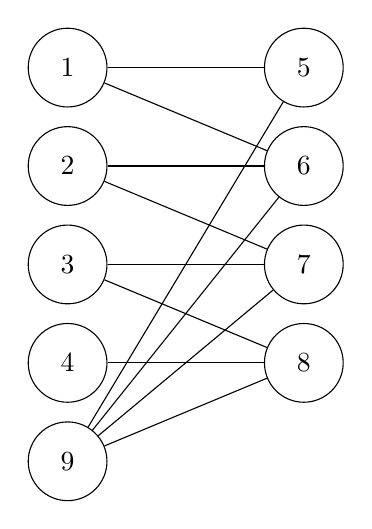
\begin{tikzpicture}[scale=1, every node/.style={draw, circle, minimum size=1cm, inner sep=2pt}]
    % Left group (partition 1)
    \node (1) at (0,5) {1};
    \node (2) at (0,3.75) {2};
    \node (3) at (0,2.5) {3};
    \node (4) at (0,1.25) {4};
    \node (9) at (0,0) {9}; 

    % Right group (partition 2)
    \node (5) at (3,5) {5};
    \node (6) at (3,3.75) {6};
    \node (7) at (3,2.5) {7};
    \node (8) at (3,1.25) {8};

    % Edges between partitions
    \draw (1) -- (5);
    \draw (1) -- (6);
    \draw (2) -- (6);
    \draw (2) -- (7);
    \draw (3) -- (7);
    \draw (3) -- (8);
    \draw (4) -- (8);
    \draw (5) -- (9);
    \draw (6) -- (9);
    \draw (7) -- (9);
    \draw (8) -- (9);
\end{tikzpicture}
\end{center}

This graph is bipartite because we can partition its vertex set into two groups:  
$\{1,2,3,4,9\}$ and $\{5,6,7,8\}$, where no edges exist within each individual group.

\babc
\item 
Describe an algorithm to determine whether a given undirected graph is bipartite and briefly justify its correctness (no formal proof necessary).
\item
Write pseudocode for your algorithm.
\item 
Analyze the time complexity of your algorithm.
\eabc


\vspace{0.5in}

\exercise 
Consider the following statement:
\begin{quote}
If $G = (V,E)$ is a directed graph, performing a breadth-first search in $G$ starting from some node $s \in V$ will return the \emph{weakly connected component} that $s$ belongs to in $G$.
\end{quote}
Explain why this statement is false. 
Then explain how to change it slightly into a statement that describes a strategy that \textit{does} use a BFS in some way to successfully find the weakly-connected component for $s$ in $G$.

\newpage
\challenge
Let $G = (V, E)$ be an undirected graph with $|V| = n$ vertices and $|E| = m$ edges.  
Each edge is colored either \textbf{red} or \textbf{blue}.  
You are given a starting vertex $s \in V$ and an integer $k \ge 0$.

Each vertex $v \in V$ has a \textbf{portal switch}. Activating the portal at $v$ flips the colors of all edges incident to $v$ (red $\leftrightarrow$ blue).  
Each portal may be activated at most once, and you may activate at most $k$ portals total during your traversal.

You begin at vertex $s$.  
You may traverse an edge only if its current color matches the color of the previously traversed edge.  
The first edge you traverse may be either color.

Your goal is to compute, for every vertex $v \in V$, the minimum number of edges needed to reach $v$ from $s$ under these rules.  
If a vertex is unreachable, report its distance as $\infty$.

\babc
\item 
Describe an algorithm that correctly computes these minimum distances.  
Clearly specify the state representation you use and explain how you enforce both the color constraint and the portal-switch constraint.

\item 
Briefly justify why your algorithm correctly finds shortest valid paths.

\item 
Write clear pseudocode for your algorithm.

\item 
Analyze the runtime of your algorithm in terms of $n$, $m$, and $k$.
\eabc
\end{document}